% file: 3-8-apsp/vt-gadget.tex

\documentclass[tikz]{standalone}
\usetikzlibrary{positioning}

\begin{document}
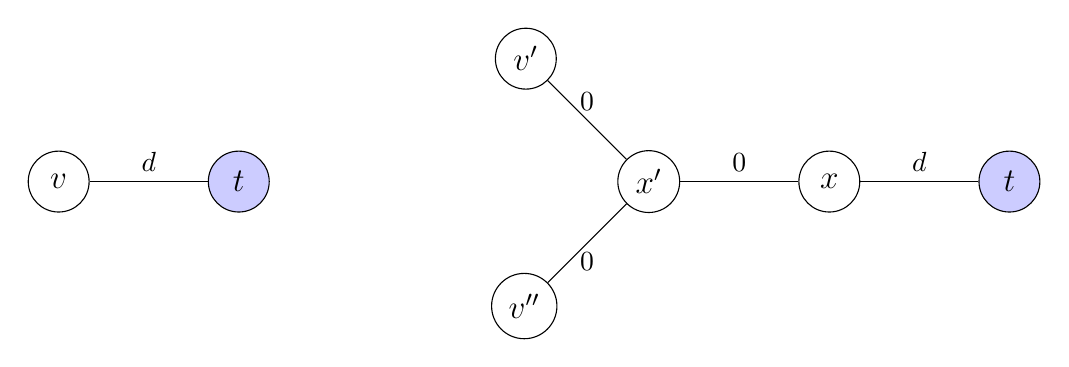
\begin{tikzpicture}[vertex/.style = {draw, circle, minimum size = 22pt, font = \large},
    node distance = 1.0 and 1.0cm,
    every edge/.style = {draw, -}]

  \node (v) [vertex] {$v$};
  \node (t) [fill = blue!20, vertex, right = 1.5cm of v] {$t$};
  \draw (v) to node [above] {$d$} (t);

  \node (t) [fill = blue!20, vertex, right = 9.0cm of t] {$t$}; % t is overwritten
  \node (x) [vertex, left = 1.5cm of t] {$x$};
  \node (x') [vertex, left = 1.5cm of x] {$x'$};

  \node (v') [vertex, above left = of x'] {$v'$};
  \node (v'') [vertex, below left = of x'] {$v''$};

  \path (t) edge node[above] {$d$} (x)
	(x) edge node[above] {$0$} (x')
	(x') edge node[above] {$0$} (v')
	     edge node[below] {$0$} (v'');
\end{tikzpicture}
\end{document}

